\chapter{Multi-channel Acoustic Pulse Recognition System}\label{ch:MultichannelAPR}

\ifpdf
    \graphicspath{{Chapter4_MultiAPR/Chapter4Figs/PNG/}{Chapter4_MultiAPR/Chapter4Figs/PDF/}{Chapter4_MultiAPR/Chapter4Figs/}{Chapter4_MultiAPR/Chapter4Figs/Training/}}
\else
    \graphicspath{{Chapter4_MultiAPR/Chapter4Figs/EPS/}{Chapter4_MultiAPR/Chapter4Figs/}}
\fi

%Introduction to multi-channel APR
While a key aspect of the basic single-channel Acoustic Pulse Recognition (APR) system was founded in the breath of devices in the market meeting the hardware requirements for the system presented in chapter~\ref{ch:APR}, a range of devices are emerging with multiple sensors, and specifically multiple microphones. Laptop computers, tablets and mobile phones frequently employ multiple microphones for noise cancellation\cite{Habets2013}\cite{Habets2012}, echo cancelation\cite{US7925007} and localisation applications\cite{US8174547}\cite{US8233353}.

In this chapter the APR system is generalised to multiple channels and results are provided to quantify the multi-channel APR system's performance in relation to a single-channel equivalent.

%outline of chapter
This chapter will begin outlining the background for the multi-channel APR system in relation to the previously discussed single-channel system. The theory behind the generalised theory will be presented after which the training procedures required will be discussed in relation to the approach taken in section~\ref{sec:APRtraining}. The method used for the evaluation of the work is outlined after which the results, discussion and conclusions are presented.

\section{Background}
%Discuss and outline the advantages of multiple channels in a physical detection application
Chapter~\ref{ch:APR} described the theory and application of a single-channel APR system. This system relied on the presence of a single transducer in or on the device for the APR application. For many devices this microphone implementation would be designed for speech recordings and design specifications may have included steps to actively reduce the impact of mechanically noise in the device. Multiple channels enable theoretically improved performance on two accounts. Firstly since the channels can be considered parallel and independent, each additional channel may be considered an independent trial with same expected results. This is particularly an advantage when the additional available channels are designed to specifically be a reference source discounting either some noise source (say background noise) or the target source (say speech). This enables a secondary detection or classification channel potentially affected to a lesser extent by either speech or other noise.

\subsection{Time of Flight (ToF)}
A second advantage of the multi-channel system is the main functional component of previous multi-channel APR systems\cite{TouchSystems2006}\cite{US7411581}. Time of Flight (ToF) or Time Delay of Arrival (TDA) or the relative time of arrival of, especially transient, events at uniquely placed receiving transducers gives an additional indication of the origin of a pulse.

Consider a tap on a surface which generates an pulse and thereby an acoustic wavefront propagating radially outwards from the point of impact. The array of microphones embedded in the surface will receive the wavefront at different times relative to their distance from the point of impact and the phase velocity. Figure~\ref{fig:ToFexample.pdf} shows an example of a surface with a wavefront's propagation and 3 microphones' relative position within the propagation pattern.

\begin{figure} %ToFexample.pdf
\begin{minipage}[b]{1.0\linewidth}
  \centering
  \centerline{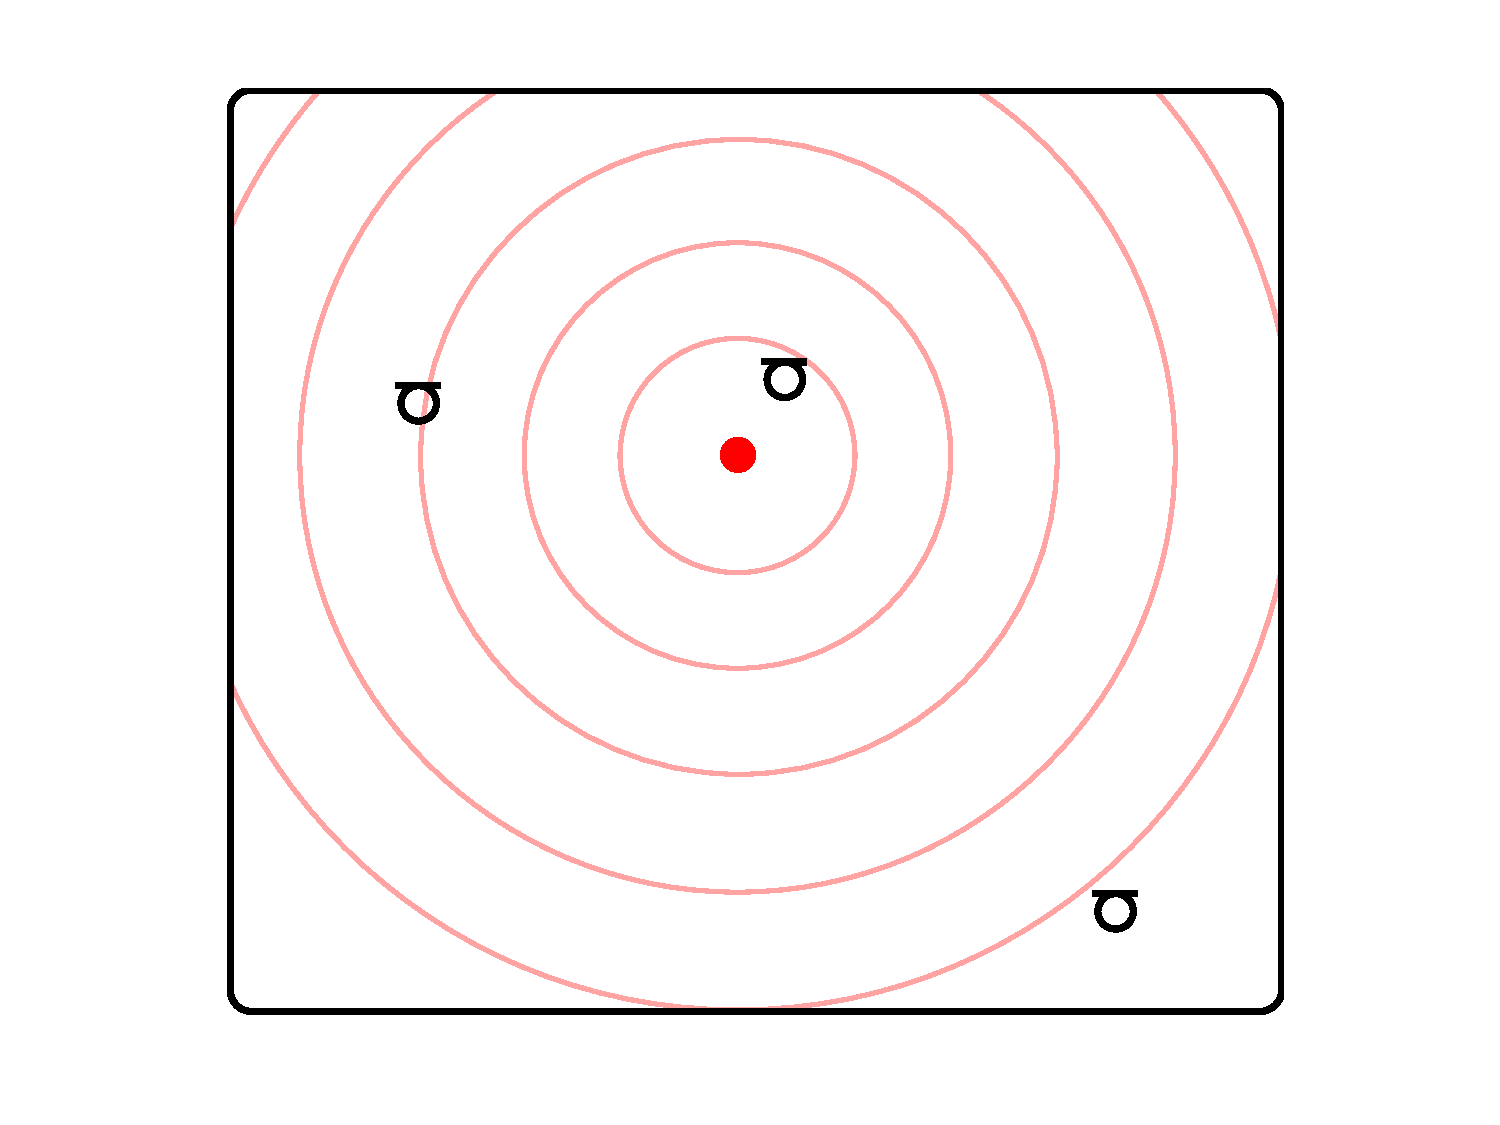
\includegraphics[width=12cm]{ToFexample.pdf}
  \begin{picture}(0,0)
\put(-200,5){Microphone}
\put(-310,5){Impact site}
\put(-80,5){Wavefront}
\end{picture}}
\end{minipage}
\caption{An example of a wavefront's radial propagation in a surface and 3 embedded microphones. All reflections are omitted.}
\label{fig:ToFexample.pdf}
\end{figure}

No timing or localisation information can be inferred from a single microphone where as a set of microphones provide a hyperbolic curve upon which the event must have occurred. No less than 3 microphones are required to locate the origin of a tap on a 2 dimensional plane\cite{US7411581}. %Figure~\ref{fig:MultiSourceExample.pdf}(a) and (b) provides an example of 3 waveforms from 3 different microphones located a different points in a system.

%Discuss time of flight (ToF) (and sample rates/size tradeoff)
For constant phase velocity $c$ in a specific material and time difference $\Delta t$ the spatial difference between microphones $\Delta d$ can be calculated with a basic equation of motion,

\begin{equation}\label{eq:ToFcalcs1}
\Delta d  = c \Delta t.
\end{equation}

For a digital system sampled at sampling rate $f_s$, time difference is equivalent to $\Delta t = \Delta S/f_s$ where $S$ is the a number of samples and $t$ and sampling rate is measured in seconds and samples per second respectively.

The positional difference $\Delta d$ can now be calculated from the sample difference $\Delta S$ between two events as,

\begin{equation}\label{eq:ToFcalcs2}
\Delta d  = c \frac{\Delta S}{f_s}.
\end{equation}

For the minimum sampling rate $f_s$ needed to detect any spatial difference $\Delta S \leq 1$ equation~\ref{eq:ToFcalcs2} is rearranged to

\begin{equation}\label{eq:ToFcalcs3}
f_s  \geq \frac{c}{\Delta d}.
\end{equation}

Figure~\ref{fig:MultiSourceExampleAnnoSpot9.pdf} shows an example of 3 waveforms from 3 different microphones embedded in a surface. Various points on the waveforms have been affixed with data tags to allow for a comparison of their relative arrival times. In this example the absolute distance in the surface from the microphones to the impact site was 30, 10 and 20 cm for microphones 1, 2 and 3 respectively. It is important to note that so far it has been the first arrivals that have been of primary concern for the positioning of signals, but Figure~\ref{fig:MultiSourceExampleAnnoSpot9.pdf} also shows other waveform elements related to the surface geometry. Microphone 3 provides a clear secondary negative peak at sample number 45. This secondary peak quite likely corresponds to a reflected (non direct) pulse arriving slightly delayed to the direct pulse due to the longer path travelled.

\begin{figure} %MultiSourceExampleAnnoSpot9.pdf
\begin{minipage}[b]{1.0\linewidth}
  \centering
  \centerline{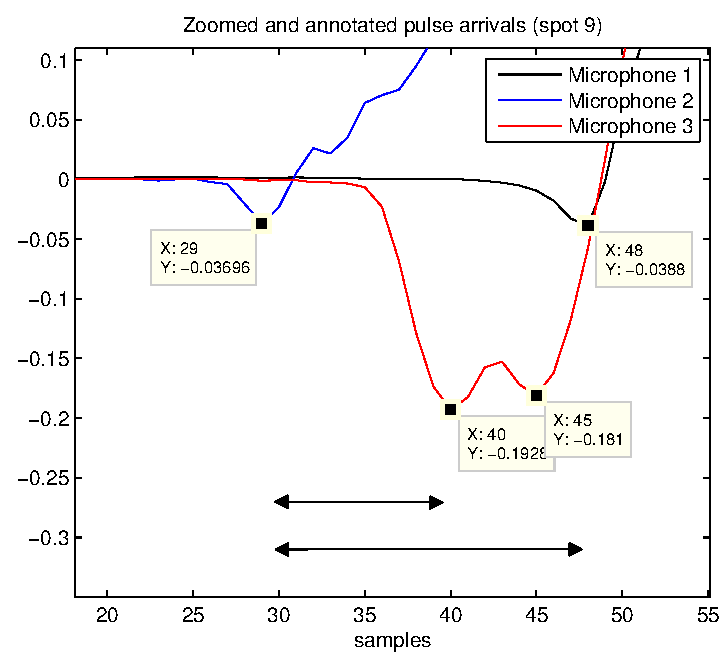
\includegraphics[width=12cm]{MultiSourceExampleAnnoSpot9.pdf}
  \begin{picture}(0,0)
\put(-180,60){11}
\put(-150,36){19}
\end{picture}}
\end{minipage}
\caption{A zoomed example of the 3 wavefronts captured, and their relative alignment, for an impact on spot 9 on the surface.}
\label{fig:MultiSourceExampleAnnoSpot9.pdf}
\end{figure}

Based on the estimated phase velocity in the surface, provided in appendix~\ref{ap:SpeedCalc}, this additional distance is 4.4 cm approximately corresponding to a range of early reflective paths on the surface.

\section{Model and theory}\label{sec:MultiAPRModelTheory}
The multi-channel model proposed here is an extension of the multi component model proposed in section~\ref{sec:APRpca}.

Similarly to equation~\ref{eq:mod1} we consider observations of the form \linebreak[0]$y_c = [y_{c,0}, \ldots , y_{c,N-1}]^T$ for the $c$th channel so that $\textbf{y} = [y_c, \ldots, y_C]$ for $C$ independent channels. The standard noisy linear instantaneous model is considered for a single-channel $c$:

\begin{equation}\label{eq:mod1_c}
y_c = \sum_{i=1}^{I} \theta_{c,i}^j t_{c,i}^j(n_0) + v_c,
\end{equation}

where $t_{c,i}^j(n_0)$ is the $j$th template for the $c$th channel, $j_c \in \{1, \ldots ,J\}$, for $I$ independent components and $\theta_{c,i}^j$ is the amplitude of the $c$th channel, $j$th spot and $i$th component. In this section the model has been assumed to be of zero mean $\mu_c^j(n_0) =0$ although this assumption could easily be avoided by adding it to the model. Take $\theta_{c,i}^j$ to be a random variable, $\Theta_c^j = [\theta_{c,1}^j,\ldots,\theta_{c,I}^j]^T$, describing the scale of each template component $i$ where

\begin{equation}\label{eq:theta_c}
\Theta_c^j \sim \mathcal{N}(\mu_{\Theta_c}^j,C_{\Theta_c}^j),
\end{equation}

and Gaussian noise to model background interference:

\begin{equation}\label{eq:noise_c}
v_{c,n} \stackrel{i.i.d.}{\sim} \mathcal{N}(0,\sigma_{v,c,n}^2).
\end{equation}

Considering this model in matrix notation:
\begin{equation}\label{eq:mod2}
y_c = \textbf{t}_c\Theta_c + \textbf{v}_c.
\end{equation}

Bayes' theorem can now be used to evaluate the joint probability of $\textbf{y}$ and $\Theta$ as

\begin{equation}\label{eq:bayes1_c}
p(\textbf{y},\Theta | j, c) = p(\textbf{y}|\Theta,j,c)p(\Theta | j,c).
\end{equation}

Since the goal is to evaluate the probability of each data reading $\textbf{y}$ given a particular position/model $j$, the dependency of $\Theta$ can be marginalized out,

\begin{eqnarray}\nonumber
p(\textbf{y}|j) &=& \int_\Theta p(\textbf{y},\Theta|j) d\Theta \\
\label{eq:marg1_c} &=& \int_\Theta p(\textbf{y}|\Theta,j)p(\Theta|j) d\Theta.
\end{eqnarray}

As with the single-channel method, see equation~\ref{eq:loglikeli}, the log-likelihood is calculated

\begin{equation}\label{eq:loglikeli_c}\begin{split}
\log{p(y_c|j)} = &- \frac{n}{2}\log{2 \pi}- \frac{1}{2}\log{|\Phi_c|} - \frac{1}{2}\log{|C_{\Theta,c}|} \\
& -\frac{1}{2\sigma^2_{v,c}}\left(\sigma_{v,c}^2\mu_\Theta^TC_{\Theta,c}^{-1}\mu_{\Theta,c} + y_c^Ty_c- \left(\Phi_c^T\right)^{-1}\Lambda_c^T\Lambda_c\right).
\end{split}\end{equation}

Since the channels are considered independent of each other we have that

\begin{equation}\label{eq:jointprob_c}
p(\textbf{y} | j) = \prod^C p(\textbf{y} | j, c).
\end{equation}

Similar to equation~\ref{eq:MLdefinition}, the Maximum Likelihood (ML) estimator can be expressed as

\begin{equation}\label{eq:MLdefinition_c}
p(j |\textbf{y}) = \argmax{j} \prod^C p(y|j,n_0,c),
\end{equation}

\begin{equation}\label{eq:MLdefinition2_c}
\log{\left( p(j |\textbf{y})\right)} = \argmax{j} \sum^C \log{\left( p(y|j,n_0,c) \right)}.
\end{equation}

\section{Training}\label{sec:MultiAPRTraining}
%describe the different training schemes employed
The training of the templates for the multi-channel APR system proceeds similarly to the single-channel APR PCA based system outlined in section~\ref{sec:APRtraining} with a few exceptions. In all tests conducted the number of PCA components used was $I = 8$.

In this chapter a number of different methods will be compared, while these will be described in more detail in section~\ref{sec:MultiAPRMethod}, the training for these models will be outlined below.

The diagram presented in Figure~\ref{fig:trainingSystem1.pdf} outlines the most basic, or the base line approach that will be tested in this chapter. Each channel $c$ will be considered independently and so the training stage will exactly mirror that presented in section~\ref{sec:MultiAPRMethod} relating to the PCA training with $J$ different templates. The right side of Figures~\ref{fig:trainingSystem1.pdf}-\ref{fig:trainingSystem3.pdf} shows an example of how various models will relate to the data when they are tested. Testing is done on $Q$ samples.

\begin{figure} %trainingSystem1.pdf
\begin{minipage}[b]{1.0\linewidth}
  \centering
  \centerline{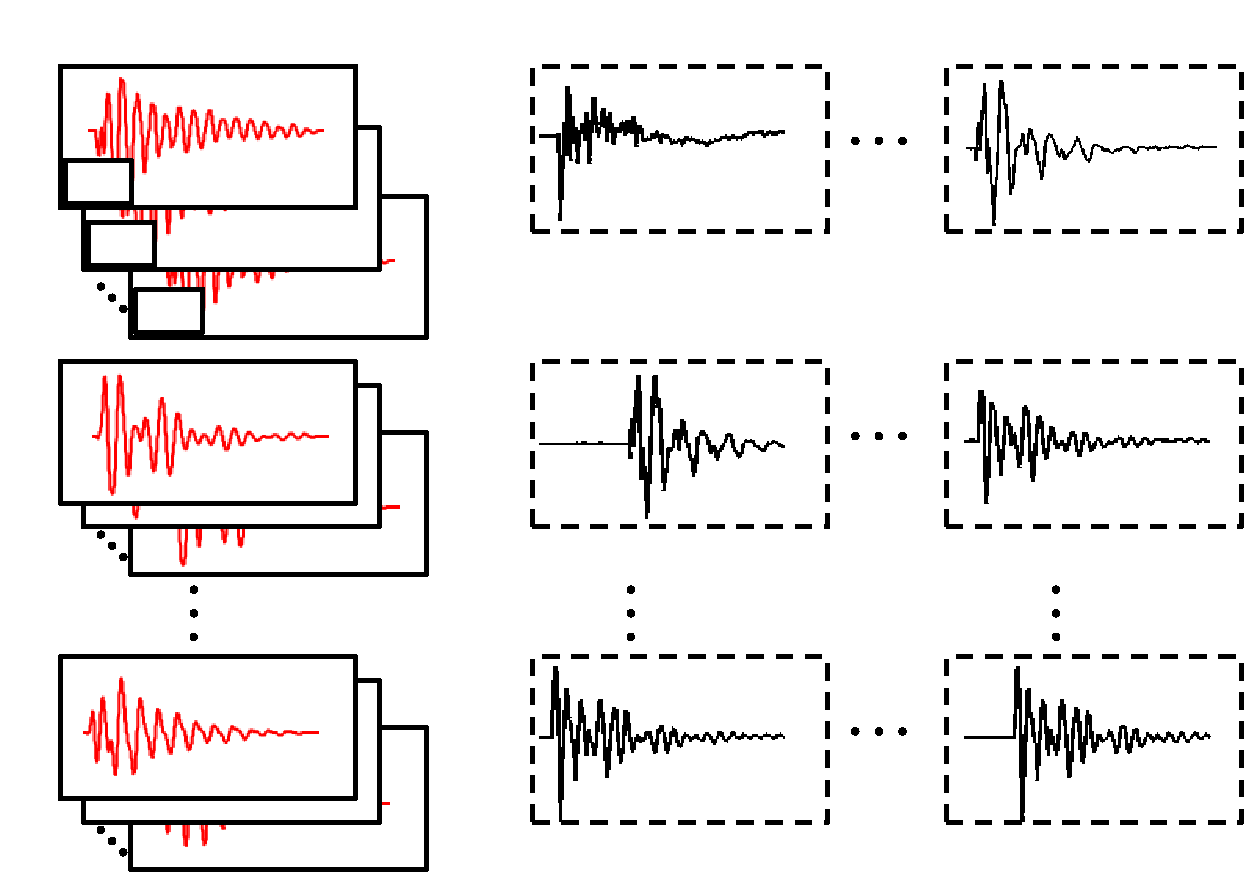
\includegraphics[width=13cm]{trainingSystem1.pdf}
  \begin{picture}(0,0)
  \put(-334,260){Training}
  \put(-133,260){Testing}
  \put(-180,250){q=1}
  \put(-60,250){q=Q}
\put(-351,205){j=1}
\put(-344,187){j=2}
\put(-329,167){j=J}
\put(-380,219){c=1}
\put(-380,129){c=2}
\put(-380,41){c=C}
\end{picture}}
\end{minipage}
\caption{Example of individual training per channel $c$ and the templates' application in testing.}
\label{fig:trainingSystem1.pdf}
\end{figure}

An initial implementation of the multi-channel system training is shown in Figure~\ref{fig:trainingSystem2.pdf}. Here the templates are considered together but aligned independently. This approach follows the training method presented in section~\ref{sec:MultiAPRMethod} and while the classification probabilities are considered jointly the templates are trained independently allowing for different templates with different lengths and number of components $I$.

\begin{figure} %trainingSystem2.pdf
\begin{minipage}[b]{1.0\linewidth}
  \centering
  \centerline{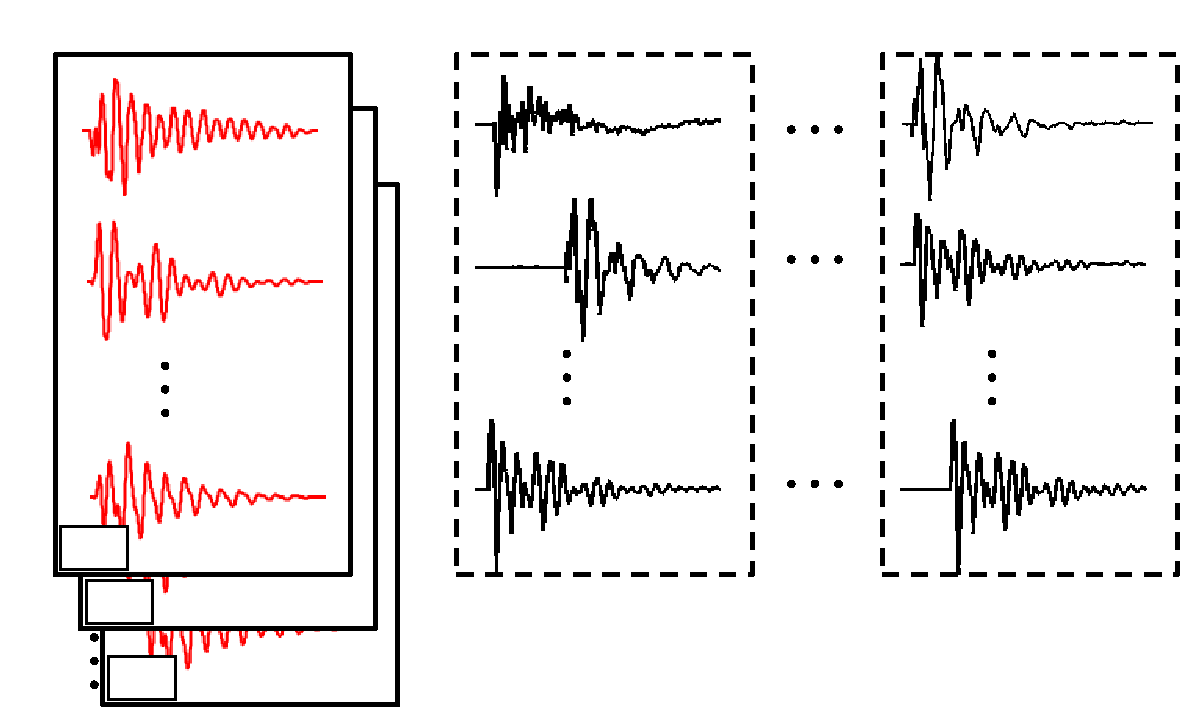
\includegraphics[width=13cm]{trainingSystem2.pdf}
  \begin{picture}(0,0)
    \put(-334,225){Training}
    \put(-137,225){Testing}
    \put(-195,215){q=1}
  \put(-65,215){q=Q}
\put(-351,50){j=1}
\put(-342,33){j=2}
\put(-334,9){j=J}
\put(-380,180){c=1}
\put(-380,133){c=2}
\put(-380,65){c=C}
\end{picture}}
\end{minipage}
\caption{Example of individually aligned training but joint probability, and the templates' application in testing.}
\label{fig:trainingSystem2.pdf}
\end{figure}

Figure~\ref{fig:trainingSystem3.pdf} shows the multi-channel APR system training using joint alignment. While, as in section~\ref{sec:MultiAPRMethod}, the other methods presented here have trained each channel independently, this approach only prompts the trainer for alignment cues based on data from one channel. This means that the relative alignments between channels $c$ and spots $j$ remain intact. Data associated with each channel can be stored independently as previously but each template will now be of similar length and will require slightly longer templates to account for pulses arriving prior to those of the alignment channel (channel 1 $c=1$ for all tests conducted).

\begin{figure} %trainingSystem3.pdf
\begin{minipage}[b]{1.0\linewidth}
  \centering
  \centerline{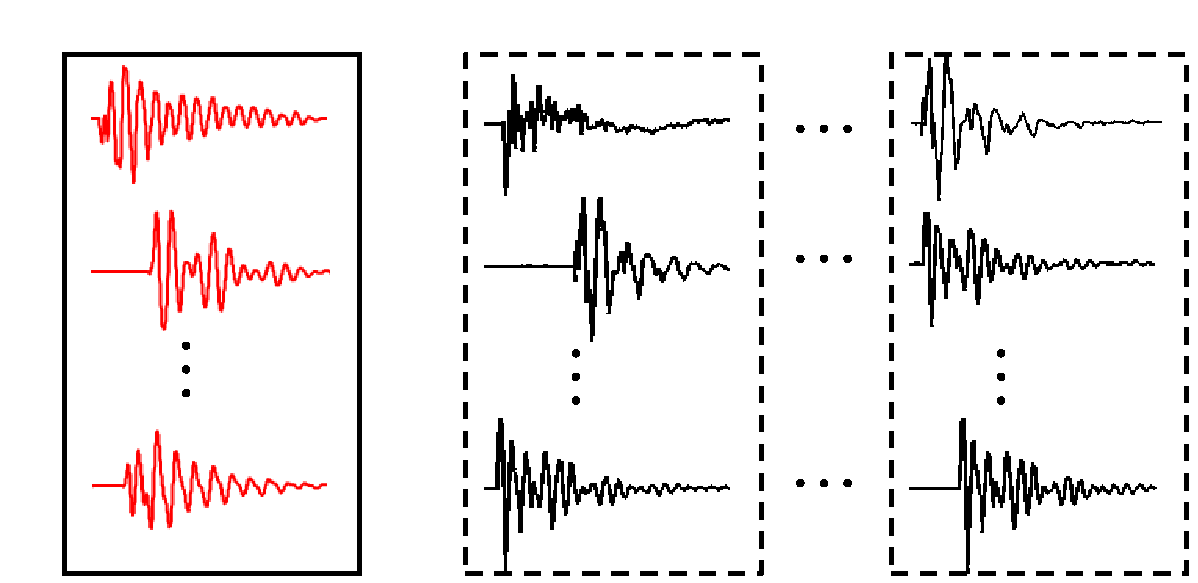
\includegraphics[width=13cm]{trainingSystem3.pdf}
  \begin{picture}(0,0)
    \put(-334,225){Training}
  \put(-137,225){Testing}
    \put(-195,215){q=1}
  \put(-65,215){q=Q}
\put(-350,49.5){j=1}
\put(-342,33){j=2}
\put(-334,9){j=J}
\put(-380,182){c=1}
\put(-380,135){c=2}
\put(-380,68){c=C}
\end{picture}}
\end{minipage}
\caption{Example of fixed alignment training, and the templates' application in testing.}
\label{fig:trainingSystem3.pdf}
\end{figure}

\section{Method}\label{sec:MultiAPRMethod}
\subsection{System setup}\label{sec:MultiAPRSystem}
To evaluate the performance of the algorithms a multi-channel setup was assembled. Figure~\ref{fig:MultiAPRsystem.pdf} shows a diagram of the system. The legend to the right indicates the elements in the diagram the numbers to the left of each microphone and active spot is the channel/microphone and active spot/template number respectively used henceforth. The surface used in this system is the same as shown in Figure~\ref{fig:Pad} but different active spots, or trained spots, have been chosen.

\begin{figure} %MultiAPRsystem.pdf
\begin{minipage}[b]{1.0\linewidth}
  \centering
  \centerline{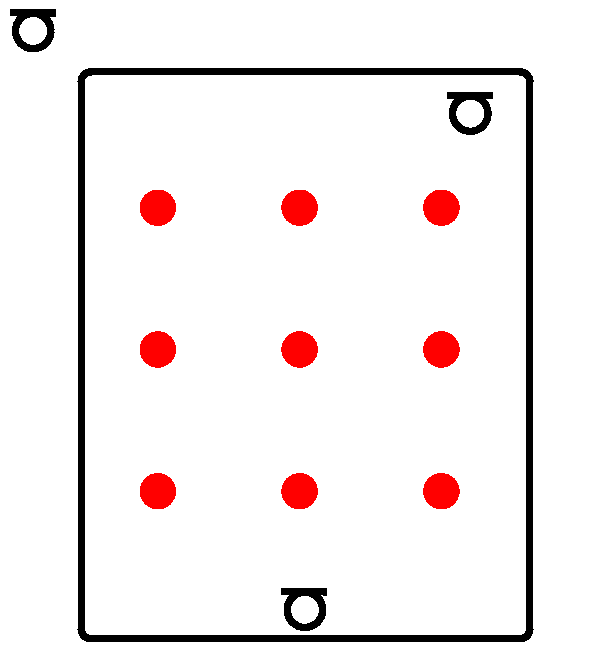
\includegraphics[width=10cm]{MultiAPRsystem.pdf}
  \begin{picture}(0,0)
\put(-90,176){Microphone}
\put(-90,158){Active spots}
\put(-90,140){Surface edge}
\put(-294,186){1}
\put(-210,8){2}
\put(-159,160){3}
\put(-253,132){1}\put(-209.5,132){2}\put(-166,132){3}
\put(-253,89){4}\put(-209.5,89){5}\put(-166,89){6}
\put(-253,45){7}\put(-209.5,45){8}\put(-166,45){9}
\end{picture}}
\end{minipage}
\caption{Diagram of testing setup with numbered microphones and active spots.}
\label{fig:MultiAPRsystem.pdf}
\end{figure}

It is noted that Microphone 1 is not embedded within the surface but is located slightly above and beyond the surface edge, whereas Microphones 2 and 3 are embedded within the back of the surface wedged in with low density foam similarly to tests conducted in section~\ref{sec:APRsystem}. Equipment details, photographs of setup and evaluation of converter accuracy is provided in appendix~\ref{ap:MultiAPRsystem}.

These differences in microphone type, placement and mounting demonstrates that the algorithm treats the system as a black box with the only requirement being reproducibility, and that any transducer could be substituted for the ones used in these experiments.

\subsection{Data}
Training data for the $J=9$ models, see Figure~\ref{fig:MultiAPRsystem.pdf}, consisted of approximately 33 seconds of audio data containing between 46 and 52 taps at varying intensity and strike angle. The taps were done with a capped Bic Cristal pen ``BiC\textregistered''. The $C=3$ channels were recorded simultaneously.

%tests Q for q=1 to q=Q
Two data sets were used for testing in this chapter, one without noise and one with noise. The noiseless set consisted of $Q=79$ testing taps and the noisy set consisted of $Q=45$ taps both were randomly distributed over the $J=9$ active spots. Each set of testing taps $q$ was comprised of $C=3$ channels. Each $Q \times C$ tapping pulse was separated into separate audio files of approximately 2 seconds length.

All data was recorded as PCM 16 bit audio data sampled at 48 kHz. The noisy testing sets were recorded with loud music playing in the background. Figure~\ref{fig:NoisyMicSignalsCompare} shows an example of an pulse recorded in a clean and in a noisy environment for microphone 1, Figure~\ref{fig:NoisyMicSignalsCompare}(a), and for microphone 2, Figure~\ref{fig:NoisyMicSignalsCompare}(b). It is clearly noted that the signal from microphone 2 is less affected by the acoustic noise. This mixture of more and less noise sensitive microphones emulates the real world scenario of devices with noise or signal reference microphones for noise reduction algorithms.

\begin{figure}[t]
\begin{minipage}[b]{1.0\linewidth}
  \centering
  \centerline{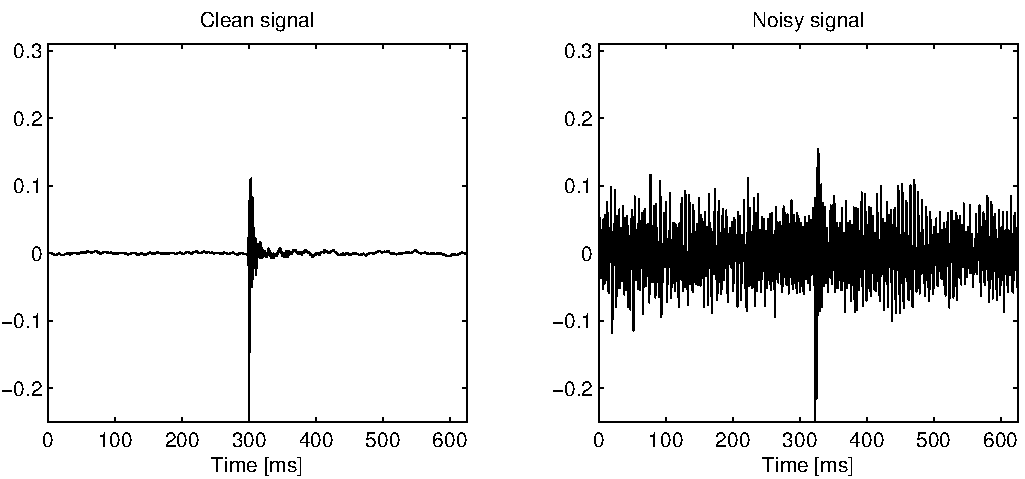
\includegraphics[width=11cm]{NoiseCompare1}}%10
  %\vspace{.5cm}
  \centerline{(a) Microphone 1 }\medskip
\end{minipage}
\begin{minipage}[b]{1.0\linewidth}
  \centering
  \centerline{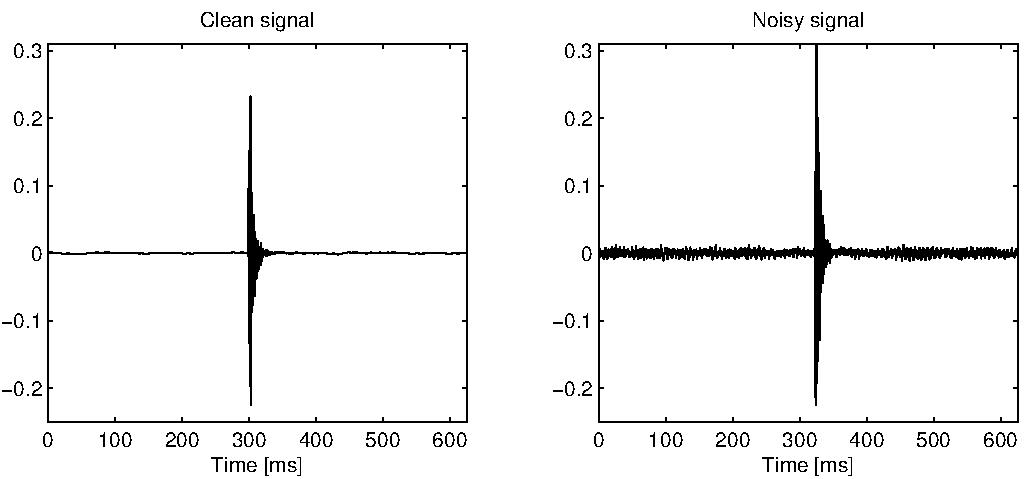
\includegraphics[width=11cm]{NoiseCompare2}}%10
  %\begin{picture}(0,0)
%\put(-120,382){(a)}
%\put(-120,195){(b)}
%\end{picture}
 %\vspace{1.5cm}
  \centerline{(b) Microphone 2}\medskip
\end{minipage}
\caption{Examples of audio signal (waveform) in clean and noisy conditions for (a) Microphone 1 and (b) Microphone 2.}
\label{fig:NoisyMicSignalsCompare}
\end{figure}

\subsection{Approaches}
While the underlying theory behind the multi-channel APR system was outlined in section~\ref{sec:MultiAPRModelTheory}, the actual implementation of decision process can be approached in various ways. This section will outline the ones for which training approaches were presented in section~\ref{sec:MultiAPRTraining} and results are presented in section~\ref{sec:MultiAPRResults}. Each approach will be given a number (Approach \#) as in aid to evaluate the results in section~\ref{sec:MultiAPRResults}.

As mentioned previously the multi-channel approach will be compared to the standard single-channel approach (\approachChFourN{app:IndiChan}). The single-channel PCA method will be run for each channel $c$ and will return a total number of $QC$ results for $Q$ tests and $C$ channels as shown in Figure~\ref{fig:trainingSystem1.pdf}. In addition the single-channel results will be processed and the unique mode (\approachChFourN{app:IndiChanMode}) for each test $q$ result, if it exists, will be shown together with the median (\approachChFourN{app:IndiChanMedian}) for each test $q$.

Figure~\ref{fig:trainingSystem2.pdf} introduced a simple naive multi-channel implementation (\approachChFourN{app:MultiNaive}). Here the channels were not aligned and the detection likelihoods were combined as described in equation~\ref{eq:MLdefinition2_c}. While this approach clearly fails to take advantage of the inherent ToF information it may serve as a control to evaluate the effect of ToF. In addition to this approach the maximum detection likelihood for each channel $c$ are combined and the class corresponding the combined largest excitation is chosen (\approachChFourN{app:MultiNaiveMax}). In other words:

\begin{equation}\label{eq:jointprob3_c}
p(j|y) = \argmax{j} \prod^C \underset{n_0}{\max} p(y|j,n_o,c).
\end{equation}

This approach attempts to remedy the naive multi-channel approach by making an assumption. It is assumed that while a template may not perfectly fit an pulse associated with a different template, it will still have its maximum excitation when aligned correctly with the pulse. This enables a \emph{post hoc} pseudo alignment of the templates. This approach is included to remedy the naive multi-channel approach.

Lastly the approach described in Figure~\ref{fig:trainingSystem3.pdf} is presented (\approachChFourN{app:Multi}). Here the ToF information is inherently retained assuming that the relative channel alignments in the testing system is kept constant between training and testing. While a template for a single-channel may score well with wrong testing data when combined with templates for other channels the effect should be blurred in time while a correct classification will have a set of matching template in addition to matching ToF information.

\section{Results}\label{sec:MultiAPRResults}
\subsection{ToF example}
While the pulse translations, due to differences in ToF between microphones, presented in the figures in section~\ref{sec:MultiAPRTraining} were exaggerated for visual clarity, the data presented in Figure~\ref{fig:ToFexample.pdf} gave an example of the typical effect of spaced out microphones on the surface. Figure~\ref{fig:MultiSourceExample.pdf} shows the complete pulse from Figure~\ref{fig:ToFexample.pdf}. Figure~\ref{sec:MultiAPRTraining}(a) clearly shows two different pulse decay envelopes for microphones 2 and 3, with microphone 3's signal appearing to decay at a slower rate and contain more energy in general.

\begin{figure} %MultiSourceExample.pdf
\begin{minipage}[b]{1.0\linewidth}
  \centering
  \centerline{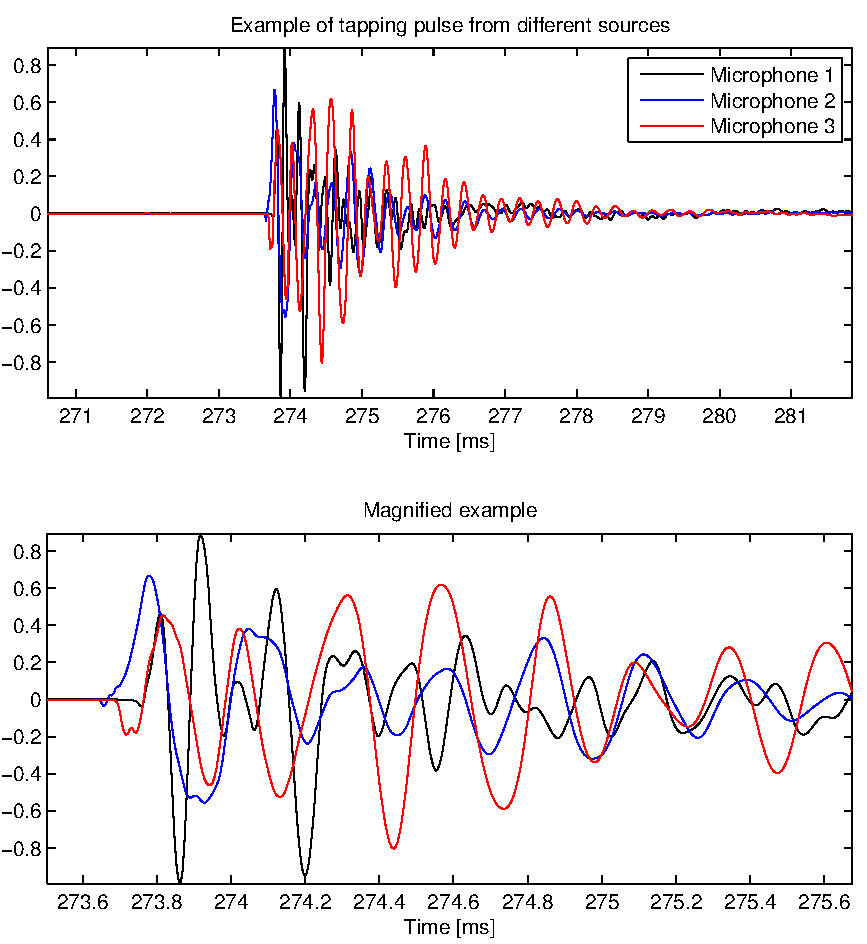
\includegraphics[width=12cm]{MultiSourceExample.pdf}
  \begin{picture}(0,0)
\put(-320,360){(a)}
\put(-320,168){(b)}
\end{picture}}
\end{minipage}
\caption{(a) An example of the 3 wavefronts captured, and their relative alignment, for an impact on spot 9 on the surface. (b) Zoomed in version of (a).}
\label{fig:MultiSourceExample.pdf}
\end{figure}

\subsection{Classification results}\label{sec:MultiAPRResultsClass}
Classification results for the multi-channel classification test are presented in Table~\ref{tab:multiAPRresults}. The expected baseline for random guessing is $11 \%$ for this 9 spot model.
\begin{table}\begin{center}
\caption{Multi-channel classification results}
\label{tab:multiAPRresults}
\begin{tabular}{|c|l|c|c|c|}\hline
Approach \#             & Approach description          & \% correct    & \% wrong  & \% missed  \\ \hline
\ref{app:IndiChan}      & Individual channels           & 89            & 11        & 0          \\
                        &  - mic 1 $c = 1$              & 99            & 1         & 0          \\
                        &  - mic 2 $c = 2$              & 77            & 23        & 0          \\
                        &  - mic 3 $c = 3$              & 90            & 10        & 0          \\
\ref{app:IndiChanMode}  & Individual channels (mode)    & 92            & 5         & 3          \\
\ref{app:IndiChanMedian}& Individual channels (median)  & 92            & 8         & 0          \\
\ref{app:MultiNaive}    & Multi-channel Independent     & 75            & 25        & 0          \\
\ref{app:MultiNaiveMax} & Multi-channel Max Probability & 94            & 6         & 0          \\
\ref{app:Multi}         & Multi-channel Joint           & 99            & 1         & 0          \\ \hline
\end{tabular}\end{center}\end{table}

The results for individual channels from Approach \ref{app:IndiChanMode} has been presented in Table~\ref{tab:multiAPRresults}. The Individually trained and tested channels approach correct classification result of $89\%$ is an average of the results from all channels. It should be noted that the individual channels are not proposed as classification methods in their own right, since all channels should be considered of equal weight. The individual channels are only presented here for transparency and to underline that Approach~\ref{app:IndiChan} was run on all test files individually.

Since all the noiseless data contained nothing that could be confused with an pulse, the detection threshold could be set to a very low level without any false detections. The missed classification results noted for the mode-based individual channel approach (Approach \ref{app:IndiChanMode}) was due to three way disagreements between the channels. It is also noted that in these missed detection cases the similar median based classification approach (Approach \ref{app:IndiChanMedian}) will simply have picked the spot with the median value in a numerical sense. The noisy data was processed with the same low threshold as in the noiseless case, but it is assumed, for both the noisy and the noiseless case, that the maximum excitation is still caused by the pulse in the audio segment.

In Table~\ref{tab:multiAPRresultsNoise} the results from at slightly smaller $Q=45$ test are presented. These results are conducted in a noisy environment with music playing in the background but with the same templates as with the previous test.

\begin{table}\begin{center}
\caption{Multi-channel classification results in noisy environment.}
\label{tab:multiAPRresultsNoise}
\begin{tabular}{|c|l|c|c|c|}\hline
Approach \#             & Approach description          & \% correct    & \% wrong  & \%  missed  \\ \hline
\ref{app:IndiChan}      & Individual channels           & 83            & 17        & 0           \\
                        &  - mic 1 $c = 1$              & 98            & 2         & 0           \\
                        &  - mic 2 $c = 2$              & 78            & 22        & 0           \\
                        &  - mic 3 $c = 3$              & 73            & 27        & 0           \\
\ref{app:IndiChanMode}  & Individual channels (mode)    & 87            & 7         & 7           \\
\ref{app:IndiChanMedian}& Individual channels (median)  & 89            & 11        & 0           \\
\ref{app:MultiNaive}    & Multi-channel Independent     & 51            & 49        & 0           \\
\ref{app:MultiNaiveMax} & Multi-channel Max Probability & 84            & 16        & 0           \\
\ref{app:Multi}         & Multi-channel Joint           & 100           & 0         & 0           \\ \hline
\end{tabular}\end{center}\end{table}


\section{Discussion}
The results presented in section~\ref{sec:MultiAPRResultsClass} show a consistently increasing classification performance for the multi-channel APR system with the best performance achieved from the aligned trained and tested multi-channel system (Approach \ref{app:Multi}) with a classification result of 99\% for the 79 clean trials and 100\% for the 45 noisy trials.

%Single-channel results perform well. Which microphone performs best is possibly a question of environment though.
With the exception of Approach~\ref{app:MultiNaive}, the poorest performance was achieved by the individually trained approach (\ref{app:IndiChan}), yet looking at the performance for channel 1 it was noted that this channel managed correct classification performance identical to Approach \ref{app:Multi} in the clean test while in the noisy test it got very close to it. As can be seen clearly in Figure~\ref{fig:NoisyMicSignalsCompare} the acoustic noise has affected microphone 1 to a larger extent than microphone 2 (and presumably 3 given their identical mounting) despite the classification results still being the best for channel 1.

Slightly improved performance, from the basic individually trained approach (\ref{app:IndiChan}), was achieved by looking at the individual channel results' mode and median values. for the $C=3$ system these approaches were identical with the exception of the case where all three channels were in disagreement. Here the mode-processed method returned class 0 indicating the relative ignorance of the result, where the median result returns the median of the classes' numerical value. In our clean data results it is noted that the 3 \% in question, equal to 2 trials, were guessed incorrectly by the median processing step. Table~\ref{tab:multiAPRresultsNoise} highlighted the difference between approaches \ref{app:IndiChanMode} and \ref{app:IndiChanMedian} with a 2 percentage point (pp) difference at the cost of a 4 pp increase in wrong classifications. It is noted that in certain situations this might be a sensible guess but in most cases it would be tantamount to a random guess between the competing methods. The sparse training scenario discussed in section~\ref{sec:APRspareTraining} could be viable candidate for the median processed classification result if eventually extended to a multi-channel scenario.

Approaches \ref{app:IndiChanMode} and \ref{app:IndiChanMedian} were presented as a way of achieving higher classification accuracy with only access to the various classes retrieved from the individual classifiers. Approaches \ref{app:MultiNaive} and \ref{app:MultiNaiveMax} present possible extensions when the underlying classifying statistics are considered as well. As predicted, Approaches \ref{app:MultiNaive} does not perform as well as the other methods due to the relatively random alignment of the templates, but as noted previously, Approach \ref{app:MultiNaiveMax} rectifies the underlying idea of the approach and increases the classification performance to 94 \% and 84 \% for clean and noisy tests respectively. As noted, this method assumes that the maximum excitation is achieved at perfect alignment for the correct model. While the multi-channel approach (\ref{app:Multi}) achieves 99 \% and 100 \% correct classification, this assumption clearly does not hold true. Approach \ref{app:MultiNaiveMax} remains the best performing approach for non-aligned templates.

The highest correct classification results, for both the clean and the noisy tests, were achieved with the multi-channel approach (\ref{app:Multi}) with combined alignment. While in the clean test this method managed results identical to results from to channel 1 from Approach~\ref{app:IndiChan}, in the noisy test the multi-channel approach (\ref{app:Multi}) managed slightly better performance, underlining that this approach can be better than the best of its constituent parts, and that the results suggest that the performance is unaffected by substantial environmental noise. It is reiterated that the individual channels in Approach~\ref{app:IndiChan} are not to be considered competing approaches individually since no objective weight is applied to these channels \emph{a priori}.

%more general implementation discussions


\section{Conclusions}
The results presented in this chapter showed a significant improvement in detection performance of the multi-channel APR system over a single-channel equivalent. In addition the full multi-channel approach (\ref{app:Multi}) outperformed other presented methods which also used the available channel data. For the data and scenario tested, the multi-channel approach (\ref{app:Multi}) appeared unaffected by loud environmental noise, while all other methods tested saw decreased classification accuracy.

While the devices tested in this and the previous chapter have been of moderate sizes, it is not unimaginable that the APR systems presented could be applied to even larger devices such as walls or tables. Increasing the physical dimensions of the device would generally reduce the energy in the pulses as the impact site moved away from the transducer thereby decreasing the SNR. In a multi-channel system, transducers could be distributed evenly around the surface edge maintaining high SNR for at least some channels. Models/templates with channels of low SNR could during training easily be registered and be removed from consideration during classification essentially defaulting to the ignorant prior for that channel-template combination.

%computational concerns X*C only (plus slightly longer templates)
Although the multi-channel approach (\ref{app:Multi}) in general requires slightly longer templates to capture the alignment of the models the computational cost of the multi-channel approach is a simple linear scaling with the number of channels $C$ making the formal big-``O'' complexity identical to that of the single-channel approach.

%Further work
\subsection{Possible future work}
%correlate noise
While the assumption of uncorrelated noise in the system holds for some cases, such as faint localised and own-noise, more significant noise, such as the background music used or speech, would be correlated across channels. Extending the proposed model to incorporate correlated noise might further increase the robustness of the model to false detections or false classifications.

%Correlate \theta in a channel internally

%The maximum log-likelihood value could have been consulted with a relative or absolute approach. It would also be possible to construct a quality metric based on the calculated statistics of the additional 6 classes not chosen by any of the channels.


%Mention possibility to implement with other sensors... not microphones. (gyroscopes, accelerometers)
To further evaluate the combined effect of the PCA based classification approach presented in chapter~\ref{ch:APR} and the multi-channel approach presented in this chapter, an additional testing approach could be devised that purely attempts to classify the testing data based on ToF information.

% ------------------------------------------------------------------------


%%% Local Variables:
%%% mode: latex
%%% TeX-master: "../thesis"
%%% End:
